\documentclass[tikz,border=10pt]{standalone}
\usepackage{tikz}
\usetikzlibrary{shapes.geometric, arrows.meta, positioning, calc, fit, backgrounds}

\begin{document}
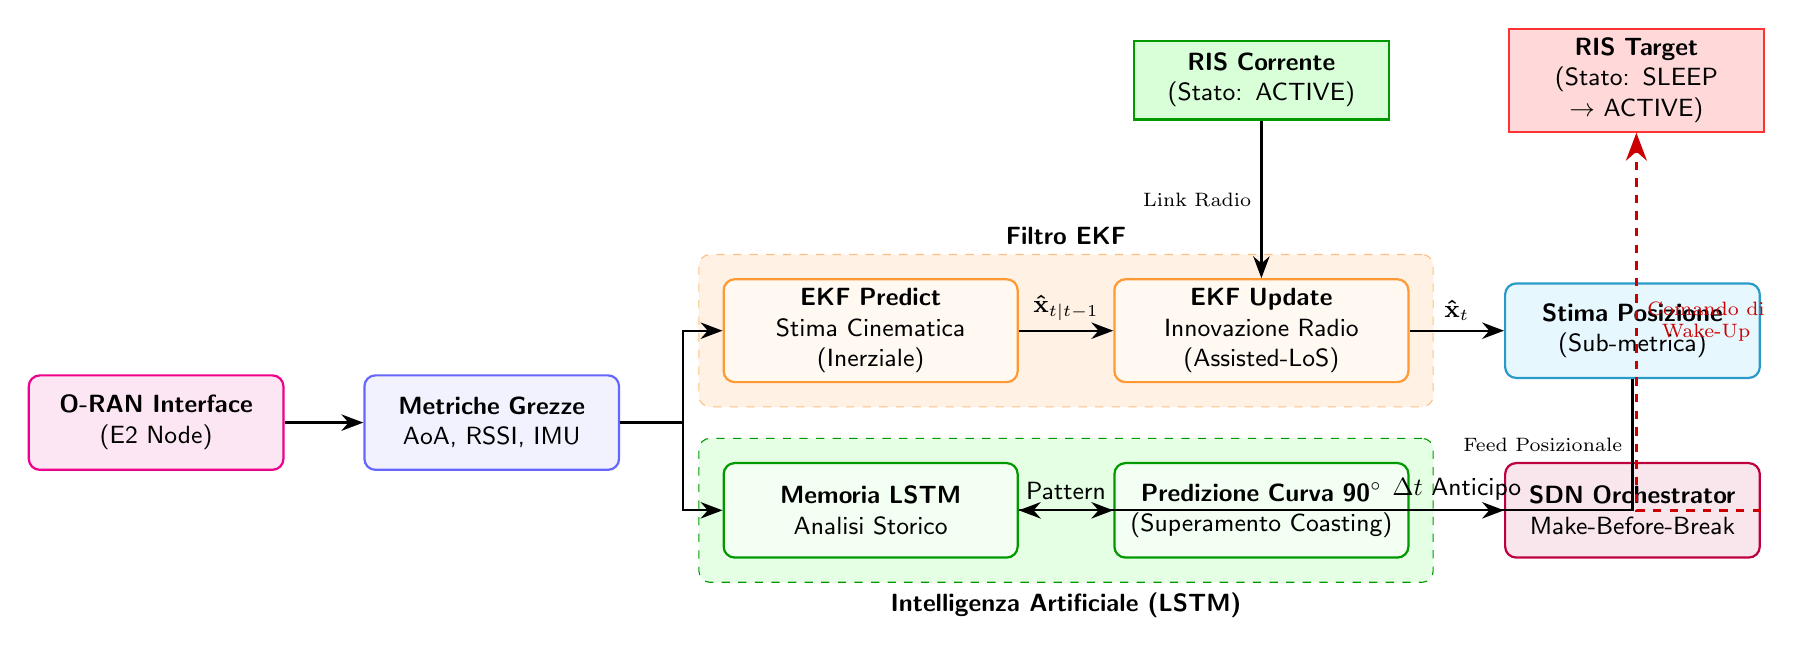
\begin{tikzpicture}[
    auto,
    font=\sffamily\small,
    block/.style = {rectangle, draw=blue!60, fill=blue!5, thick, text width=3cm, text centered, rounded corners, minimum height=1.2cm},
    ai_block/.style = {rectangle, draw=green!60!black, fill=green!5, thick, text width=3.5cm, text centered, rounded corners, minimum height=1.2cm},
    ekf_block/.style = {rectangle, draw=orange!80, fill=orange!5, thick, text width=3.5cm, text centered, rounded corners, minimum height=1.2cm},
    hardware/.style = {rectangle, draw=gray!80, fill=gray!10, thick, text width=3cm, text centered, minimum height=1cm},
    line/.style = {draw, thick, ->, -{Stealth[scale=1.2]}},
    dashed_line/.style = {draw, thick, dashed, ->, -{Stealth[scale=1.2]}},
    background_ekf/.style = {rectangle, fill=orange!10, rounded corners, draw=orange!50, dashed, inner sep=0.3cm},
    background_lstm/.style = {rectangle, fill=green!10, rounded corners, draw=green!60!black, dashed, inner sep=0.3cm}
]

% Nodes
\node [block, fill=magenta!10, draw=magenta] (oran) {\textbf{O-RAN Interface}\\(E2 Node)};
\node [block, right=1cm of oran] (telemetry) {\textbf{Metriche Grezze}\\AoA, RSSI, IMU};

\node [coordinate, right=0.8cm of telemetry] (split) {};

% EKF Path (Top)
\node [ekf_block, above right=0.5cm and 0.5cm of split] (ekf_predict) {\textbf{EKF Predict}\\Stima Cinematica\\(Inerziale)};
\node [ekf_block, right=1.2cm of ekf_predict] (ekf_update) {\textbf{EKF Update}\\Innovazione Radio\\(Assisted-LoS)};

\node [block, right=1.2cm of ekf_update, fill=cyan!10, draw=cyan!80!black] (position) {\textbf{Stima Posizione}\\(Sub-metrica)};

% LSTM Path (Bottom)
\node [ai_block, below right=0.5cm and 0.5cm of split] (lstm) {\textbf{Memoria LSTM}\\Analisi Storico};
\node [ai_block, right=1.2cm of lstm] (predict_curve) {\textbf{Predizione Curva 90$^\circ$}\\(Superamento Coasting)};

\node [block, right=1.2cm of predict_curve, fill=purple!10, draw=purple] (ris_ctrl) {\textbf{SDN Orchestrator}\\Make-Before-Break};

% Backgrounds
\begin{scope}[on background layer]
    \node[background_ekf, fit=(ekf_predict) (ekf_update), label=above:\textbf{Filtro EKF}] (ekf_bg) {};
    \node[background_lstm, fit=(lstm) (predict_curve), label=below:\textbf{Intelligenza Artificiale (LSTM)}] (lstm_bg) {};
\end{scope}

% Hardware interaction
\node [hardware, above=2cm of ekf_update, fill=green!15, draw=green!60!black] (ris_active) {\textbf{RIS Corrente}\\(Stato: ACTIVE)};
\node [hardware, right=1.5cm of ris_active, fill=red!15, draw=red!80] (ris_next) {\textbf{RIS Target}\\(Stato: SLEEP $\rightarrow$ ACTIVE)};

% Edges
\path [line] (oran) -- (telemetry);
\path [draw, thick] (telemetry) -- (split);
\path [line] (split) |- (ekf_predict);
\path [line] (split) |- (lstm);

\path [line] (ekf_predict) -- node {$\mathbf{\hat{x}}_{t|t-1}$} (ekf_update);
\path [line] (ekf_update) -- node {$\mathbf{\hat{x}}_t$} (position);

\path [line] (lstm) -- node {Pattern} (predict_curve);
\path [line] (predict_curve) -- node {$\Delta t$ Anticipo} (ris_ctrl);

% Cross interactions
\path [line] (position) |- node[near start, left, font=\scriptsize] {Feed Posizionale} (lstm);
\path [line] (ris_active) -- node[left, font=\scriptsize] {Link Radio} (ekf_update);
\path [dashed_line, color=red!80!black, very thick] (ris_ctrl) -| node[near end, right, font=\scriptsize, align=center] {Comando di\\Wake-Up} (ris_next);

\end{tikzpicture}
\end{document}
